\documentclass[aspectratio=169]{beamer}
\usetheme{Szeged}
\usecolortheme{beaver}

\usepackage{fontspec}              % Support non-latin characters
\setmonofont{Source Code Pro}%     % Select Source Code Pro for listings
            [Scale=MatchLowercase, % Adjust glyph size
             BoldFont={* Semibold}]% The Bold face is too bold

\usepackage{listings}              % Code blocks
\lstset{language={[ISO]C++},       % Default programming language
        breaklines=true,           % Break long lines in listings
        showstringspaces=false,    % Do not use visible spaces in strings
        morekeywords={constexpr,   % C++11 keywords
            decltype,static_assert}}

\usepackage{tikz}                  % TikZ drawings
\usepackage{pgfplots}
\pgfplotsset{width=12cm,height=6.5cm}
\usepackage{microtype}             % Enable black magic

\title{Proposing a Replacement for FreeBSD's powerd (Preview)}
\subtitle{Or, how I tamed the fan of my notebook}

\author[D. Fandrey]{Dominic Fandrey}
\institute[VLI]{Von Leitner-Institut für verteiltes Echtzeit-Java}
\date[GPN 2016]{GPN16, May 2016}
\logo{
\includegraphics[width=1.5cm]{logo}}

\begin{document}

\section{Introduction}

\begin{frame}[plain]
\titlepage
\end{frame}

\begin{frame}{Contents}
\tableofcontents
\end{frame}

\section{What?}

\begin{frame}{CPU p-state control}
\centering
\begin{tikzpicture}
\begin{axis}[
	xtick={5,10,15,20,25,30,35},
	x tick label style={rotate=45,anchor=east},
	ytick={0,25,50,75,100},
	ymin=0,ymax=200,
	scaled ticks=false,
	xlabel={t (s)},
	legend style={font=\tiny},
	legend pos=north west
]
\addplot[red,mark=*,mark size=.5pt] table[x=t,y=load] {../data/demo-powerd++};
\legend{load (\%)}
\end{axis}
\begin{axis}[
	xtick={100},
	ymin=-1400, ymax=3000,
	ytick={2400,2000,1600,1200,800},
	yticklabel pos=right,
	legend style={font=\tiny}
]
\addplot[jump mark right,blue]  table[x=t,y=freq] {../data/demo-powerd++};
\addplot+[red!50!blue,mark=*,mark options={fill=red!50!blue},mark size=.5pt]
        table[x=t,y=want] {../data/demo-powerd++};
\legend{cpu0 (MHz),wanted (MHz)}
\end{axis}
\end{tikzpicture}
\end{frame}

\section{Why?}
\section{How?}

\begin{frame}{powerd}
\centering
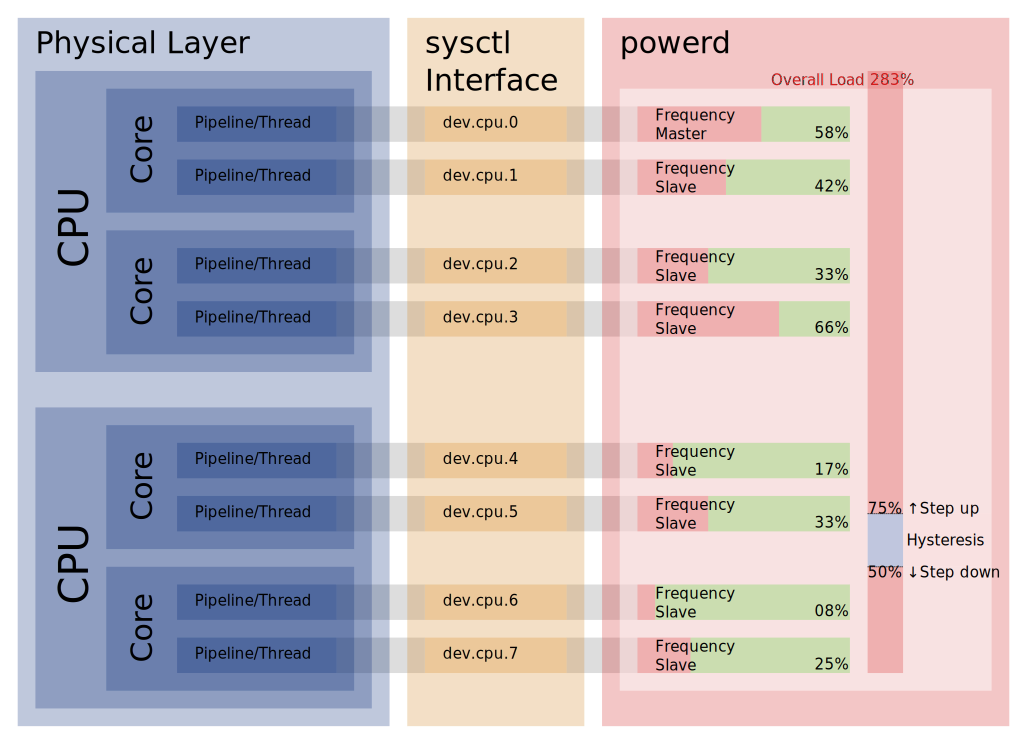
\includegraphics[height=6.5cm]{arch_powerd}
\end{frame}

\begin{frame}{powerd++}
\centering
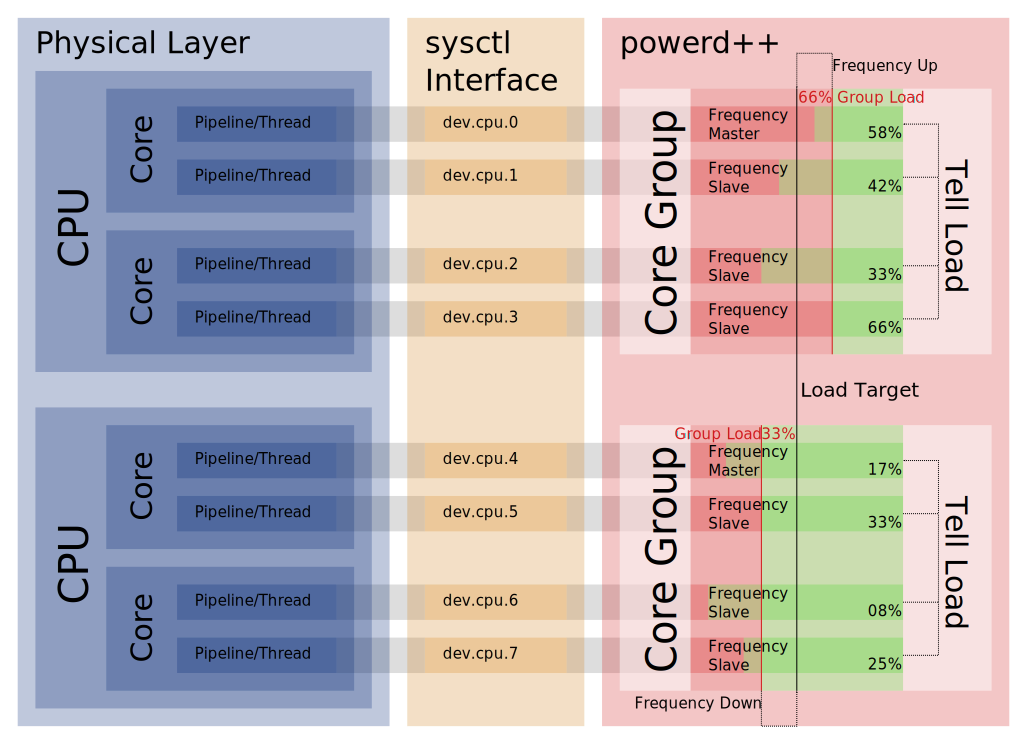
\includegraphics[height=6.5cm]{arch_powerd++}
\end{frame}

\end{document}
